\subsection{UC8 - Selezione scaffalatura}
\begin{figure}[H]
  \centering
  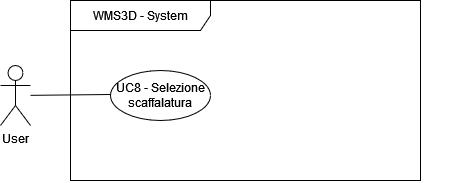
\includegraphics[width=0.8\textwidth]{UC_diagrams_1-10/UC8_sys.drawio.png}
   \caption{Diagramma UML UC8 - Selezione scaffalatura}
\end{figure}
\begin{figure}[H]
  \centering
  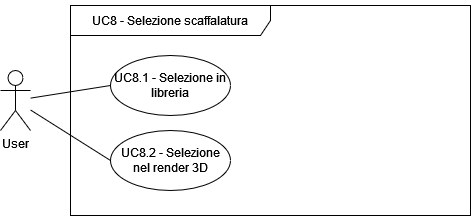
\includegraphics[width=0.8\textwidth]{UC_diagrams_1-10/UC8.drawio.png}
   \caption{Diagramma UML in dettaglio UC8 - Selezione scaffalatura}
\end{figure}
\begin{itemize}
    \item \textbf{Attori:} User.
    \item \textbf{Pre-condizione:}  L'utente ha posizionato una scaffalatura [UC7] e la sta visualizzando nel render 3D [UC3.2] e nella libreria [UC4.1.1].
    \item \textbf{Post-condizione:} La scaffalatura presa in considerazione dall'utente viene selezionata ed evidenziata.
    \item \textbf{Scenario Principale:} L'utente seleziona la scaffalatura e, indipendentemente da dove la seleziona, questa verrà selezionata sia nella libreria [UC8.1] sia nel render 3D [UC8.2].
    \item \textbf{Generalizzazioni:} -
    \item \textbf{Estensioni:} -
\end{itemize}


\subsubsection{UC8.1 - Selezione scaffalatura in libreria}
\begin{figure}[H]
  \centering
  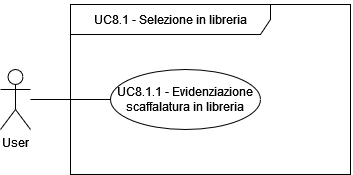
\includegraphics[width=0.8\textwidth]{UC_diagrams_1-10/UC8.1.drawio.png}
   \caption{Diagramma UML UC8.1 - Selezione scaffalatura in libreria}
\end{figure}
\begin{itemize}
    \item \textbf{Attori:} User.
    \item \textbf{Pre-condizione:} L'utente ha posizionato una scaffalatura [UC7] e la visualizza nella libreria [UC4.1.1].
    \item \textbf{Post-condizione:} La scaffalatura presa in considerazione dall'utente viene selezionata ed evidenziata nella libreria.
    \item \textbf{Scenario Principale:} L'utente seleziona la scaffalatura, la quale viene selezionata in libreria ed evidenziata in essa [UC8.1.1].
    \item \textbf{Generalizzazioni:} -
    \item \textbf{Estensioni:} -
\end{itemize}


\subsubsection{UC8.1.1 - Evidenziazione scaffalatura in libreria}
\begin{itemize}
    \item \textbf{Attori:} User.
    \item \textbf{Pre-condizione:} L'utente ha selezionato una scaffalatura [UC8].
    \item \textbf{Post-condizione:} La scaffalatura selezionata viene evidenziata in libreria.
    \item \textbf{Scenario Principale:} La scaffalatura selezionata viene evidenziata in libreria.
    \item \textbf{Generalizzazioni:} -
    \item \textbf{Estensioni:} -
\end{itemize}


\subsubsection{UC8.2 - Selezione scaffalatura in render 3D}
\begin{figure}[H]
  \centering
  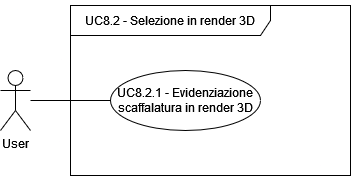
\includegraphics[width=0.8\textwidth]{UC_diagrams_1-10/UC8.2.drawio.png}
   \caption{Diagramma UML UC8.2 - Selezione scaffalatura in render 3D}
\end{figure}
\begin{itemize}
    \item \textbf{Attori:} User.
    \item \textbf{Pre-condizione:} L'utente ha posizionato una scaffalatura [UC7] e la visualizza nel render 3D.
    \item \textbf{Post-condizione:} La scaffalatura presa in considerazione dall'utente viene selezionata ed evidenziata nel render 3D.
    \item \textbf{Scenario Principale:} L'utente seleziona la scaffalatura, la quale viene selezionata nel render 3D ed evidenziata in esso [UC8.2.1].
    \item \textbf{Generalizzazioni:} -
    \item \textbf{Estensioni:} -
\end{itemize}


\subsubsection{UC8.2.1 - Evidenziazione scaffalatura in render 3D}
\begin{itemize}
    \item \textbf{Attori:} User.
    \item \textbf{Pre-condizione:} L'utente ha selezionato una scaffalatura [UC8].
    \item \textbf{Post-condizione:} La scaffalatura selezionata viene evidenziata nel render 3D.
    \item \textbf{Scenario Principale:} La scaffalatura selezionata viene evidenziata nel render 3D.
    \item \textbf{Generalizzazioni:} -
    \item \textbf{Estensioni:} -
\end{itemize}